\chapter{Implementación básica de Path Tracing}
	
En este capítulo se procede a dar un esquema básico de los fundamentos de este algoritmo. El objetivo será así describir un motor de renderizado previo a cualquier optimización, que cuenta con las funcionalidades básicas para producir una imagen de una escena tridimensional simple.


\section{Esquema Path Tracing}
\label{pathtracingexplanation}


	\subsection{Aproximación de la ecuación de renderizado}
\[
{\displaystyle L_{\text{o}}(\mathbf {x} ,\omega _{\text{o}})=L_{\text{e}}(\mathbf {x} ,\omega _{\text{o}})\ +\int _{\Omega }f_{\text{r}}(\mathbf {x} ,\omega _{\text{i}},\omega _{\text{o}})L_{\text{i}}(\mathbf {x} ,\omega _{\text{i}})(\omega _{\text{i}}\cdot \mathbf {n} )\operatorname {d} \omega _{\text{i}}}
\]

La Ecuación de Renderizado \cite{kajiya1986rendering} aparece por primera vez en 1986 junto al algoritmo de Path Tracing, siendo este algoritmo una propuesta para resolverla. Es el pilar de la visualización 3d fotorrealista ya que simula de una manera suficientemente precisa la interacción de la luz en una escena tridimensional. En este trabajo se utiliza una interpretación más moderna que sustituye términos como el "término geométrico" y adapta dicha ecuación al estado del arte.

La interpretación de esta ecuación es la siguiente: Para un punto $\mathbf {x}$ del espacio y un ángulo $\omega _{\text{o}}$ desde el cual se observa a dicho punto, cuál es la cantidad de energía lumínica que el observador recibe $L_{\text{o}}$.

El primer término $L_{\text{e}}(\mathbf {x} ,\omega _{\text{o}})$ indica la luz que dicho punto $\mathbf {x}$ emite, así pues se podrán modelar materiales que emitan luz propia y no dependan de energía externa.

El segundo término calcula toda la luz entrante y reflejada a través del ángulo $\omega _{\text{o}}$ por dicho punto $\mathbf {x}$, es por ello que integra todos los ángulos del hemisferio superior. Este segundo término se compone de tres coeficientes:

El primer coeficiente $f_{\text{r}}(\mathbf {x} ,\omega _{\text{i}},\omega _{\text{o}})$ es la función BRDF, la cual es dependiente del material e indica cuánta energía se refleja en dicho punto para las direcciones de entrada $\omega _{\text{i}}$ y salida $\omega _{\text{o}}$.

El segundo coeficiente $L_{\text{i}}(\mathbf {x} ,\omega _{\text{i}})$ hace referencia a toda la energía lumínica entrante de todas las direcciones posibles.

El tercer coeficiente $(\omega _{\text{i}}\cdot \mathbf {n})$ es el producto de la ley del coseno de Lambert \cite{lambert1760jh}, un escalar que atenúa los ángulos menos pronunciados con la normal de la superficie.

\begin{figure}[H]
    \centering
	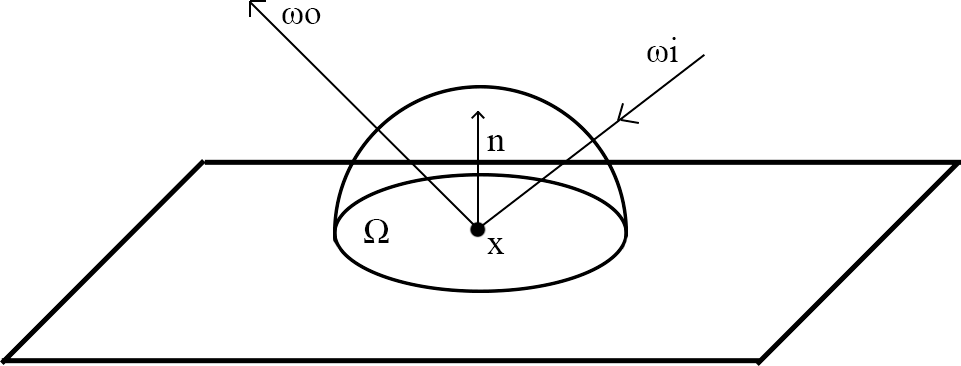
\includegraphics[width=0.5\textwidth]{renderingequation}
	\caption{Interpretación geométrica del término de integración la ecuación de renderizado}
	\label{fig:label}
\end{figure}


	\subsection{Esquema de resolución}
	\label{subsec:montecarlo}
Kajiya \cite{kajiya1986rendering} propone junto a la ecuación, el algoritmo de Path Tracing para resolverla. Este algoritmo se fundamenta en el método de Monte Carlo debido a la imposibilidad de resolver dicha ecuación de manera analítica.
Para aproximar una integral con el método de Monte Carlo, basta con muestrear aleatoriamente la función, y tras varias muestras es posible aproximar dicha integral. En la práctica, estas muestras son rayos con direcciones aleatorias y se tratará de aproximar la ecuación de renderizado. 

\[
{\int _{\Omega }f_{\text{r}}(\mathbf {x} ,\omega _{\text{i}},\omega _{\text{o}})L_{\text{i}}(\mathbf {x} ,\omega _{\text{i}})(\omega _{\text{i}}\cdot \mathbf {n} )\operatorname {d} \omega _{\text{i}} \approx \displaystyle \frac{1}{N}\sum\limits_{k=1}^{N}\frac{f_{\text{r}}(\mathbf {x} ,\omega _{\text{k}},\omega _{\text{o}})L_{\text{k}}(\mathbf {x} ,\omega _{\text{k}})(\omega _{\text{k}}\cdot \mathbf {n} )\operatorname {d} \omega _{\text{k}}}{p(\omega _{\text{k}})}}
\]

Así pues el procedimiento general es el siguiente:

\begin{enumerate}
	\item \hyperref[sec:calculatecameraray]{Calcular un rayo inicial desde la posición de la cámara a cada píxel del sensor de la cámara}.
	\item \hyperref[sec:throwray]{''Lanzar'' dicho rayo a la escena}.
	\item \hyperref[subsec:triintersection]{Comprobar la intersección de este rayo con el elemento más cercano al origen de este}. En caso de no intersecar se entiende que el rayo ha salido de la escena, de manera que se añade la luz del fondo a dicho camino y se salta al punto.
	\item Aplicar la reducción de energía pertinente a dicha intersección.
	\item Comprobar si se ha alcanzado el número máximo de rebotes, en caso negativo se calcula la dirección a la que rebota dicho rayo y se vuelve al paso 2.
	\item Se añade al píxel la luz que contiene dicho rayo.
\end{enumerate}

\begin{figure}[H]
    \centering
	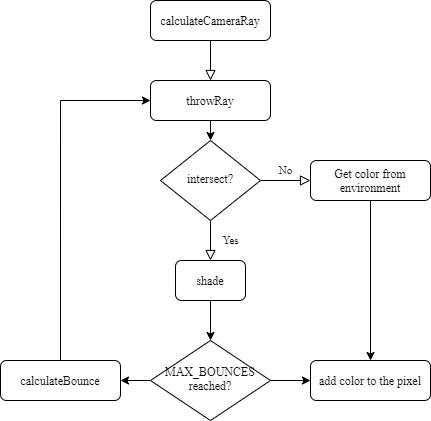
\includegraphics[width=0.5\textwidth]{algorithmscheme}
	\caption{Esquema Path Tracing}
	\label{fig:algorithmscheme}
\end{figure}



	\section{Pipeline}
		
En primer lugar es apropiado dar una visión de la estructura que se ha programado para Eleven Rendererer. Esta estructura está formada por una serie de clases y procedimientos cuyo objetivo es simular una escena 3D, transferirla a la GPU, ejecutar el algoritmo, transferir de vuelta el resultado como una imagen final y por último mostrar esta imagen al usuario. Además se ofrecerán distintas métricas con el fin de evaluar y conocer el estado del algoritmo para determinada escena.

\subsection{Preparado de escena}

El primer paso es preparar la escena a renderizar \code{Scene}. Una escena básica se compone de una cámara \code{Camera}, geometrías \code{MeshObject} y materiales \code{Material}.

La clase \code{Scene} contiene un array dinámico para cada conjunto de elementos, con sus pertinentes funciones de añadido. Por ejemplo, la función \code{addMeshObject()} lleva la cuenta de objetos en la escena y actualiza el ID de cada objeto a partir de esta cuenta. Además esta clase cuenta con una función denominada \code{Scene sceneBuilder(std::string path)} que cargará una escena localizada en un directorio. Más detalles sobre el formato de estas escenas se puede encontrar en \hyperref[sceneformat]{el manual ubicado en el anexo}

Los elementos básicos que almacena una escena son los siguientes:

\begin{itemize}

\item Cámaras \code{Camera}: consisten en una simulación aproximada de una cámara física real, así pues sus atributos serán: tamaño del sensor (en metros) \code{sensorWidth} y \code{sensorHeight}, distancia focal (en metros) \code{focalLength} y resolución (en píxeles) \code{xRes} e \code{yRes}. 

\item Geometrías \code{MeshObject}: son elementos que contienen un conjunto de triángulos \code{Tri} los cuales a su vez consisten en 3 puntos tridimensionales \code{Vector3 vertices[3]}.

\item Materiales \code{Material}: definen la manera en la que los fotones interactúan con ellos. En su forma más primitiva consisten en un color base, el cual absorberá ciertas longitudes de onda en mayor o menor medida. Para simplificar las computaciones, no es necesario calcular estas interacciones con todo el espectro electromagnético visible, basta con usar los tres colores primarios aditivos: rojo, verde y azul, así pues un color consiste en un vector \code{Vector3(R,G,B)}.

\end{itemize}

Una vez preparada la escena se inicia el proceso de renderizado. La función \code{startRender} prepara dos buffers en la CPU, \code{rawPixelBuffer} que recibirá los píxeles procedentes del algoritmo, previos a cualquier modificación y \code{beautyBuffer} que contendrá la imagen final preparada para ser mostrada en pantalla. 


El siguiente paso es transferir la escena a la GPU, donde se realizará el resto de computaciones más demandantes. Esto es realizado por la función \code{renderSetup}, que a través de las funciones de la API de CUDA \code{cudaMalloc} y \code{cudaMemcpy} copia la información de la escena y lleva la cuenta de la memoria transferida en las variables globales \code{textureMemory, geometryMemory}. La copia de memoria de la CPU a la GPU requiere de un tratado especial en cuanto a objetos con atributos refiere, requiriendo así una copia profunda de los atributos en formato array o punteros, además de un proceso posterior denominado ''pointer binding''. Este proceso como se aprecia en la \autoref{fig:pointerbinding} es necesario puesto que los objetos que hacen referencias a punteros al ser copiados a la GPU pierden dicha referencia al cambiar de contexto. 

Para ello si un objeto \code{Object} contiene un atributo \code{int* array}, habrá que asignar espacios de memoria diferentes para cada uno, copiar ambos independientemente y posteriormente, a través de la función \code{cudaMemcpy}, copiar la dirección del array a la dirección del atributo.

\code{cudaMemcpy(\&(Object->array), \&(array), sizeof(array*), cudaMemcpyHostToDevice);}

\begin{figure}[H]
    \centering
	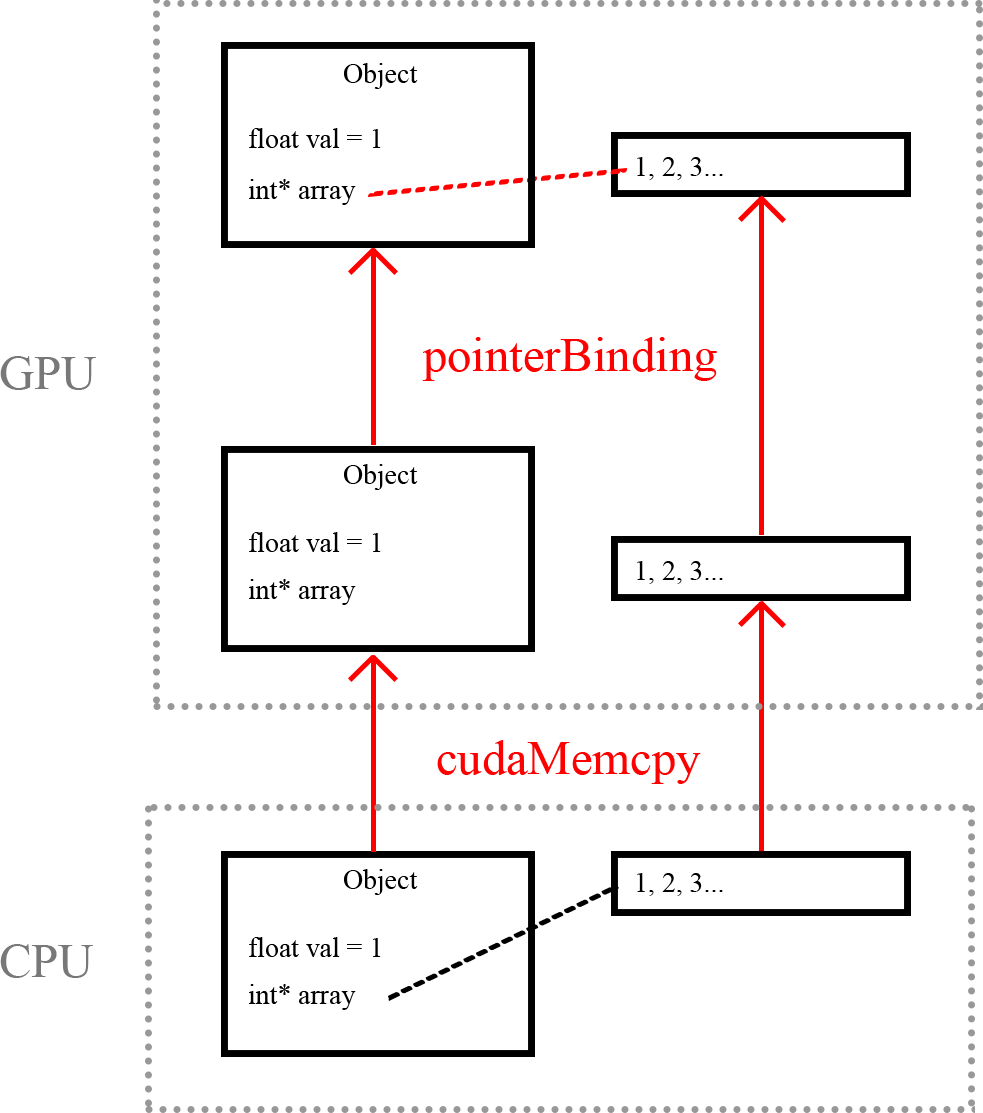
\includegraphics[width=0.5\textwidth]{pointerbinding}
	\caption{Pointer Binding}
	\label{fig:pointerbinding}
\end{figure}


La función \code{startRender}, tras realizar toda la copia de los elementos a la GPU, ejecuta un kernel que configura algunos parámetros iniciales. Este kernel \code{setupKernel} se ejecuta de manera síncrona y se hace cargo de inicializar los bufferes de píxeles y contador de rayos, inicializar \code{curand} (la librería utilizada para generar números aleatorios en CUDA) y por último, enlazar cada \code{MeshObject} con sus pertinentes triángulos. Esto es llevado a cabo con un puntero a una posición de la lista global de triángulos, ya que por motivos que posteriormente se explican en \hyperref[BVH]{Estructuras de Aceleración} es conveniente almacenar todos los triángulos por separado. 



\begin{lstlisting}
	
	__global__ void setupKernel() {

		int x = threadIdx.x + blockIdx.x * blockDim.x;
		int y = threadIdx.y + blockIdx.y * blockDim.y;

		int idx = (dev_scene_g->camera->xRes * y + x);

		if ((x >= dev_scene_g->camera->xRes) || (y >= dev_scene_g->camera->yRes)) return;

		dev_samples[idx] = 0;
		dev_pathcount[idx] = 0;

		cudaMemset(&dev_buffer[4 * idx], 0, sizeof(float) * 3); // RGB channels
		dev_buffer[4 * idx + 3] = 1; // Alpha channel

		curand_init(0, idx, 0, &d_rand_state_g[idx]);

		// Just one thread
		if (x == 0 && y == 0) {
			int triSum = 0;
			for (int i = 0; i < dev_scene_g->meshObjectCount; i++) {
				dev_scene_g->meshObjects[i].tris += triSum;
				triSum += dev_scene_g->meshObjects[i].triCount;
			}
		}
	}
\end{lstlisting}
	
Una vez la escena está correctamente configurada en la GPU, se crea un hilo nuevo que ejecutará en bucle el kernel de renderizado tantas iteraciones como muestras se hayan definido en los parámetros \code{RenderParameters}. Es necesario el uso de la librería \code{std::thread} para este proceso, ya que este bucle de llamadas a la GPU es un proceso bloqueante. El uso de dos hilos, uno para la ejecución de los kernels de renderizado y otro para la recolección de datos de la GPU de manera asíncrona, permite una previsualización dinámica del resultado del motor. Más detalles sobre este proceso se describen en el apartado \hyperref[progressiverender]{Renderizado Progresivo}.

En este punto, el algoritmo está ejecutándose en la GPU. Para mostrar el resultado se crea una ventana con la librería multiplataforma \code{SFML}. Esta librería permite mostrar en pantalla una imagen en formato RGB de 8 bits. Para poder adaptar el resultado del algoritmo a una imagen visible es necesario aplicar una serie de funciones de postprocesado. \code{getRenderData} se encarga de aplicar estas funciones y obtener una imagen postprocesada visible, también conocida en informática gráfica como "Beauty Pass".

Las funciones a ejecutar de postprocesado son las siguientes:

\begin{enumerate}
	
	\item \code{flipY}: Debido a la configuración de la cámara, los píxeles son calculados de abajo a arriba, es necesario entonces invertirlos en el eje Y.
	\item \code{clampPixels}: Es la forma más sencilla de mapeo de tonos, limitar los valores al rango [0-1].
	\item \code{applysRGB}: Los monitores no trabajan en un espacio de color lineal, por eso es necesario aplicar la curva de correción de gamma 2.2.
	\item \code{HDRtoLDR}: Por último es necesario convertir el array de píxeles de punto flotante a bytes. Una simple multiplicación por 255 hace el trabajo.

\end{enumerate}

Finalmente la librería de \code{SFML} se encarga de mostrar la imagen y superpone un texto con el número de muestras calculadas hasta el momento, obtenidas con \code{getSamples}

\section{Acumulado de muestras}
	
Puesto que el añadir la luz a un píxel puede sonar ambiguo, se acompaña el código hecho para la acumulación de muestras. \code{dev\_samples[]} es una variable global que almacena un contador con el número de muestras acumuladas hasta el momento para un píxel determinado.

\[{pixelAccumulatedLight * \frac{samples}{samples + 1} + \frac{newLight}{samples + 1}}\]

\begin{lstlisting}
	
	unsigned int sa = dev_samples[idx]; // sa is the number of samples accumulated for this pixel.
	
	if (!isnan(light.x) && !isnan(light.y) && !isnan(light.z)) {

        if (sa > 0) {
            dev_buffer[4 * idx + 0] *= ((float)sa) / ((float)(sa + 1));
            dev_buffer[4 * idx + 1] *= ((float)sa) / ((float)(sa + 1));
            dev_buffer[4 * idx + 2] *= ((float)sa) / ((float)(sa + 1));
        }

        dev_buffer[4 * idx + 0] += light.x / ((float)sa + 1);
        dev_buffer[4 * idx + 1] += light.y / ((float)sa + 1);
        dev_buffer[4 * idx + 2] += light.z / ((float)sa + 1);

        dev_samples[idx]++;
    }
	
\end{lstlisting}

El uso de la función \code{isnan} se ha determinado que es necesario para evitar errores numéricos tras encontrar artefactos gráficos en determinadas escenas. 
	
\subsection{Renderizado Progresivo}
\label{progressiverender}
		
	Una ventaja de los motores de renderizado más modernos es el renderizado progresivo. Esto implica que las muestras se van acumulando poco a poco a lo largo de la imagen hasta que terminan por converger. Esto difiere de los motores de renderizado por CPU tradicionales, que acumulan las muestras en secciones locales y una vez que acumulan las suficientes, pasan a la siguiente sección. Se ha decidido hacer una implementación progresiva con el fin de estar más cerca del estado del arte.
	
	Este tipo de implementación se beneficia de la copia de datos asíncrona de la GPU. Mientras el kernel se ejecuta, un flujo de datos secundario hará la copia del buffer de la GPU en la CPU, pudiendo así actualizar la visualización del resultado varias veces por segundo.

	Este flujo de datos secundario se ha implementado con el tipo de datos \code{cudastream\_t} de la API de CUDA. Han sido necesarios dos flujos, uno denominado \code{kernelStream} y otro denominado \code{bufferStream}. Los kernels de inicialización y renderizado correrán en el primero, mientras que la función que obtiene el buffer, será lanzada en el segundo.
	
	La función que extrae el buffer de píxeles de la GPU a la CPU es la siguiente:
	
	\begin{lstlisting}
	cudaError_t getBuffer(float* pixelBuffer, int* pathcountBuffer, int size) {

		cudaStreamCreate(&bufferStream);

		cudaError_t cudaStatus = cudaMemcpyFromSymbolAsync(pixelBuffer, dev_buffer, size * sizeof(float) * 4, 0, cudaMemcpyDeviceToHost, bufferStream);
		if (cudaStatus != cudaSuccess) {
			fprintf(stderr, "returned error code %d after launching addKernel!\n", cudaStatus);
		}

		cudaStatus = cudaMemcpyFromSymbolAsync(pathcountBuffer, dev_pathcount, size * sizeof(unsigned int), 0, cudaMemcpyDeviceToHost, bufferStream);
		if (cudaStatus != cudaSuccess) {
			fprintf(stderr, "returned error code %d after launching addKernel!\n", cudaStatus);
		}

		return cudaStatus;
	}
	\end{lstlisting}
	
	Hace uso de la función \code{cudaMemcpyFromSymbolAsync} para realizar la copia asíncrona antes mencionada. También se hace copia del buffer de la suma de rayos emitidos por píxel con el fin de realizar métricas de eficiencia.
	
	%@todo analisis de movimiento de datos de memoria.


\section{Trazado de rayo desde la cámara}
\label{sec:calculatecameraray}

Para simular el trazado del rayo desde la cámara hasta la escena, se simula de manera simplificada como haría una cámara estenopeica. Para cada píxel del sensor se calcula su posición en el espacio a partir del tamaño del sensor. Esto quiere decir que el píxel (0,0) se encuentra en la esquina inferior izquierda de la ubicación física del sensor y el píxel (\code{xRes, yRes}) se encuentra en la esquina superior derecha. Puesto que no se está teniendo en cuenta la rotación de la cámara, la coordenada z del sensor se puede simplificar con la distancia de la cámara hasta el sensor.

Si se observa un sensor físico real se puede ver como los píxeles del sensor tienen un área. En la anterior explicación se determina la posición de cada píxel pero es necesario muestrear a lo largo de todo el área del píxel para simular la realidad, no solo el centro de cada uno. Es por ello que se añade un término aleatorio \code{rx, ry} que se encargará de distribuir las posiciones a lo largo de la zona de cada píxel.

\begin{lstlisting}
	
__device__ void calculateCameraRay(int x, int y, Camera& camera, Ray& ray, float r1, float r2) {

    // Relative coordinates for the point where the first ray will be launched
    float dx = camera.position.x + ((float)x) / ((float)camera.xRes) * camera.sensorWidth;
    float dy = camera.position.y + ((float)y) / ((float)camera.yRes) * camera.sensorHeight;

    // Absolute coordinates for the point where the first ray will be launched
    float odx = (-camera.sensorWidth / 2.0) + dx;
    float ody = (-camera.sensorHeight / 2.0) + dy;

    // Random part of the sampling offset so we get antialiasing
    float rx = (1.0 / (float)camera.xRes) * (r1 - 0.5) * camera.sensorWidth;
    float ry = (1.0 / (float)camera.yRes) * (r2 - 0.5) * camera.sensorHeight;

    // Sensor point, the point where intersects the ray with the sensor
    float SPx = odx + rx;
    float SPy = ody + ry;
    float SPz = camera.position.z + camera.focalLength;

    // The initial ray is created from the camera position to the sensor point. No rotation is taken into account.
    ray = Ray(camera.position, Vector3(SPx, SPy, SPz) - camera.position);
}

\end{lstlisting}

\section{Intersección en la escena}
\label{sec:throwray}

Una vez se conoce el rayo primario que se lanza desde la cámara, es necesario determinar con qué objeto colisiona y la información de esa intersección. Esto es realizado por la función \code{throwRay} que de forma ingenua se probará si el rayo intersecciona con cada triángulo de la escena y devolverá la intersección más cercana al origen del rayo. Posteriormente en \autoref{BVH} se explica un método para evitar tener que probar a intersecar cada triángulo.

\subsection{Intersección triángulo - rayo}
\label{subsec:triintersection}
	
El cálculo de la intersección de un rayo con un triángulo es una de las operaciones más fundamentales de este algoritmo. Esta operación toma como parámetros un triángulo \code{Tri} y un rayo \code{Ray} y ofrece como resultado si dicho triángulo y rayo intersecan en el espacio y además un objeto \code{Hit} el cual cuenta con información adicional de la intersección.

La información adicional que devuelve esta operación es la siguiente:

\begin{itemize}
	
	\item \code{int hit.objectID}: ID del objeto al que pertenece dicho triángulo.
	
	\item \code{Vector3 hit.position}: Posición en el espacio del punto de intersección entre el rayo y el triángulo.
	
	\item \code{Vector3 hit.normal}: Normal de la superficie, calculada a partir del producto vectorial de dos aristas del triángulo.
	
	\item \code{bool hit.valid}: Validez de una intersección, por defecto falso. Verdadero en caso de haber intersecado correctamente.

\end{itemize}

Para la implementación se ha hecho uso del algoritmo Fast Minimum Storage Ray/Triangle Intersection\cite{moller1997fast}. En este paper se explica detalladamente el algoritmo de intersección, mientras este trabajo se limita a implementar dicho algoritmo a partir de una adaptación de la implementación en C que el autor ofrece.
	
\begin{lstlisting}
	
__host__ __device__ inline bool hit(Ray& ray, Hit& hit) {

float EPSILON = 0.0000001;

        Vector3 edge1 = vertices[1] - vertices[0];
        Vector3 edge2 = vertices[2] - vertices[0];

        Vector3 pvec = Vector3::cross(ray.direction, edge2);

        float u, v, t, inv_det;

        float det = Vector3::dot(edge1, pvec);

        inv_det = 1.0 / det;

        if (det > -EPSILON && det < EPSILON) return false;

        Vector3 tvec = ray.origin - vertices[0];

        u = Vector3::dot(tvec, pvec) * inv_det;
        if (u < 0.0 || u > 1.0)
            return false;

        Vector3 qvec = Vector3::cross(tvec, edge1);
        v = Vector3::dot(ray.direction, qvec) * inv_det;
        if (v < 0.0 || (u + v) > 1.0)
            return false;

        t = Vector3::dot(edge2, qvec) * inv_det;

        if (t < 0) return false;

        Vector3 geomPosition = ray.origin + ray.direction * t;
		Vector3 geomNormal = Vector3::cross(edge1, edge2).normalized();
		
		hit.normal = geomNormal;
		hit.position = geomPosition;
		hit.valid = true;
		hit.objectID = objectID;

        return true;

\end{lstlisting}

\subsection{Kernel principal}
	
El kernel de renderizado \code{renderingKernel} se encarga de ejecutar el algoritmo descrito en la \autoref{fig:algorithmscheme}, donde el número máximo de rebotes es una constante definida en tiempo de compilación como \code{MAX\_BOUNCES}.

La ejecución de un kernel en CUDA debe estar acompañada de dos parámetros: el número de bloques y el número de hilos. En este caso, los bloques estánd distribuidos uniformemente a lo largo de la imagen como bloques bidimensionales de \code{THREADSIZE * THREADSIZE} píxeles. Resulta interesante conocer el número de hilos óptimo por cada bloque, por esa razón se han evaluado distintos tamaños de bloque en la \autoref{fig:threadsize}

\begin{lstlisting}
	
    int tx = THREADSIZE;
    int ty = THREADSIZE;

    dim3 numBlocks(scene->camera.xRes / tx + 1, scene->camera.yRes / ty + 1);
    dim3 threadsPerBlock(tx, ty);
	
\end{lstlisting}


\begin{figure}[H]
\label{fig:threadsize}
\centering
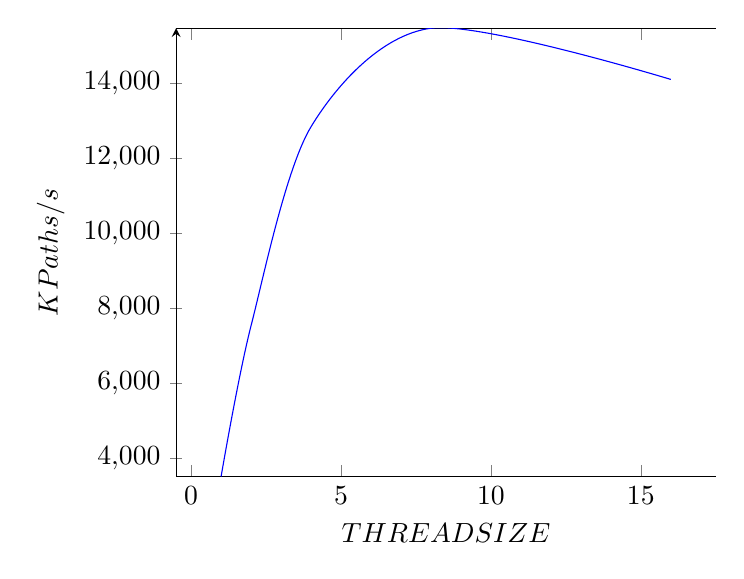
\begin{tikzpicture}
\begin{axis}[
    axis y line = left,
    xlabel = \(THREADSIZE\),
    ylabel = {\(KPaths/s\)},
	scaled y ticks=false
]

\addplot[smooth, blue]
coordinates{(1,3517) (2, 7544) (4, 12851) (8, 15480) (16, 14114)};
\end{axis}
\end{tikzpicture}
\end{figure}

